% -*- Mode:TeX -*-

%% IMPORTANT: The official thesis specifications are available at:
%%            http://libraries.mit.edu/archives/thesis-specs/
%%
%%            Please verify your thesis' formatting and copyright
%%            assignment before submission.  If you notice any
%%            discrepancies between these templates and the 
%%            MIT Libraries' specs, please let us know
%%            by e-mailing thesis@mit.edu

%% The documentclass options along with the pagestyle can be used to generate
%% a technical report, a draft copy, or a regular thesis.  You may need to
%% re-specify the pagestyle after you \include  cover.tex.  For more
%% information, see the first few lines of mitthesis.cls. 

%\documentclass[12pt,vi,twoside]{mitthesis}
%%
%%  If you want your thesis copyright to you instead of MIT, use the
%%  ``vi'' option, as above.
%%
%\documentclass[12pt,twoside,leftblank]{mitthesis}
%%
%% If you want blank pages before new chapters to be labelled ``This
%% Page Intentionally Left Blank'', use the ``leftblank'' option, as
%% above. 

\documentclass[12pt,twoside]{mitthesis}
\usepackage[spanish,es-tabla,es-noquoting]{babel} % Idioma y codificación del texto
\usepackage[utf8x]{inputenc} % Codificación del archivo
\usepackage{hyperref}
\hypersetup{%
    colorlinks=true
}
\usepackage{tikz}
\usepackage{pgfplots}
\pgfplotsset{%
    /pgf/number format/use comma,
    /pgf/number format/set thousands separator = {},
}
\usepackage[justification=centering]{caption}
\usepackage{framed}

%\usepackage{draftwatermark}
%\SetWatermarkText{DRAFT}
%\SetWatermarkScale{5}
%\SetWatermarkColor[rgb]{0.97,0.97,0.97}


%% La tipografía tiene que soportar tildes, no todas lo hacen %%
\usepackage{courier}    % Courier para tipografía monoespaciada
\usepackage{lmodern}
\usepackage[T1]{fontenc}
 
%% Si se usa hyperref + utf8x para establecer el título, autor, etc... %%
\PrerenderUnicode{á}
\PrerenderUnicode{é}
\PrerenderUnicode{í}
\PrerenderUnicode{ó}
\PrerenderUnicode{ú}
\PrerenderUnicode{ñ}

\usepackage{lgrind}
%% These have been added at the request of the MIT Libraries, because
%% some PDF conversions mess up the ligatures.  -LB, 1/22/2014
\usepackage{cmap}
\usepackage[T1]{fontenc}

%% Citas con un formato más moderno
\usepackage[square]{natbib}

\pagestyle{plain}

\begin{document}

% -*-latex-*-
% 
% For questions, comments, concerns or complaints:
% thesis@mit.edu
% 
%
% $Log: cover.tex,v $
% Revision 1.8  2008/05/13 15:02:15  jdreed
% Degree month is June, not May.  Added note about prevdegrees.
% Arthur Smith's title updated
%
% Revision 1.7  2001/02/08 18:53:16  boojum
% changed some \newpages to \cleardoublepages
%
% Revision 1.6  1999/10/21 14:49:31  boojum
% changed comment referring to documentstyle
%
% Revision 1.5  1999/10/21 14:39:04  boojum
% *** empty log message ***
%
% Revision 1.4  1997/04/18  17:54:10  othomas
% added page numbers on abstract and cover, and made 1 abstract
% page the default rather than 2.  (anne hunter tells me this
% is the new institute standard.)
%
% Revision 1.4  1997/04/18  17:54:10  othomas
% added page numbers on abstract and cover, and made 1 abstract
% page the default rather than 2.  (anne hunter tells me this
% is the new institute standard.)
%
% Revision 1.3  93/05/17  17:06:29  starflt
% Added acknowledgements section (suggested by tompalka)
% 
% Revision 1.2  92/04/22  13:13:13  epeisach
% Fixes for 1991 course 6 requirements
% Phrase "and to grant others the right to do so" has been added to 
% permission clause
% Second copy of abstract is not counted as separate pages so numbering works
% out
% 
% Revision 1.1  92/04/22  13:08:20  epeisach

% NOTE:
% These templates make an effort to conform to the MIT Thesis specifications,
% however the specifications can change.  We recommend that you verify the
% layout of your title page with your thesis advisor and/or the MIT 
% Libraries before printing your final copy.
\title{An Optimizing Compiler for Low-Level Floating Point Operations}

\author{Lucien William Van Elsen}
% If you wish to list your previous degrees on the cover page, use the 
% previous degrees command:
%       \prevdegrees{A.A., Harvard University (1985)}
% You can use the \\ command to list multiple previous degrees
%       \prevdegrees{B.S., University of California (1978) \\
%                    S.M., Massachusetts Institute of Technology (1981)}
\department{Department of Electrical Engineering and Computer Science}

% If the thesis is for two degrees simultaneously, list them both
% separated by \and like this:
% \degree{Doctor of Philosophy \and Master of Science}
\degree{Bachelor of Science in Computer Science and Engineering}

% As of the 2007-08 academic year, valid degree months are September, 
% February, or June.  The default is June.
\degreemonth{June}
\degreeyear{1990}
\thesisdate{May 18, 1990}

%% By default, the thesis will be copyrighted to MIT.  If you need to copyright
%% the thesis to yourself, just specify the `vi' documentclass option.  If for
%% some reason you want to exactly specify the copyright notice text, you can
%% use the \copyrightnoticetext command.  
%\copyrightnoticetext{\copyright IBM, 1990.  Do not open till Xmas.}

% If there is more than one supervisor, use the \supervisor command
% once for each.
\supervisor{William J. Dally}{Associate Professor}

% This is the department committee chairman, not the thesis committee
% chairman.  You should replace this with your Department's Committee
% Chairman.
\chairman{Arthur C. Smith}{Chairman, Department Committee on Graduate Theses}

% Make the titlepage based on the above information.  If you need
% something special and can't use the standard form, you can specify
% the exact text of the titlepage yourself.  Put it in a titlepage
% environment and leave blank lines where you want vertical space.
% The spaces will be adjusted to fill the entire page.  The dotted
% lines for the signatures are made with the \signature command.
\maketitle

% The abstractpage environment sets up everything on the page except
% the text itself.  The title and other header material are put at the
% top of the page, and the supervisors are listed at the bottom.  A
% new page is begun both before and after.  Of course, an abstract may
% be more than one page itself.  If you need more control over the
% format of the page, you can use the abstract environment, which puts
% the word "Abstract" at the beginning and single spaces its text.

%% You can either \input (*not* \include) your abstract file, or you can put
%% the text of the abstract directly between the \begin{abstractpage} and
%% \end{abstractpage} commands.

% First copy: start a new page, and save the page number.
\cleardoublepage
% Uncomment the next line if you do NOT want a page number on your
% abstract and acknowledgments pages.
% \pagestyle{empty}
\setcounter{savepage}{\thepage}
\begin{abstractpage}
% $Log: abstract.tex,v $
% Revision 1.1  93/05/14  14:56:25  starflt
% Initial revision
% 
% Revision 1.1  90/05/04  10:41:01  lwvanels
% Initial revision
% 
%
%% The text of your abstract and nothing else (other than comments) goes here.
%% It will be single-spaced and the rest of the text that is supposed to go on
%% the abstract page will be generated by the abstractpage environment.  This
%% file should be \input (not \include 'd) from cover.tex.
En esta tesina diseñé e implementé un servidor y varios clientes que permiten
programar robots didácticos de forma remota compartiendo un único enlace
físico entre el servidor y los robots y visualizar los movimientos de los
mismos también de forma remota. El servidor implementa un protocolo de capa
de aplicación en base a objetos JSON a través de una conexión WebSocket que
permite a los clientes interactuar con distintos modelos de robots con gran
flexibilidad, moverlos y acceder a los valores de sus sensores, además de
facilitar la visualización de los mismos a través de streaming de video.
Implementé clientes en Javascript (a ser usado desde el navegador),
Python y Ruby que permiten que este proyecto sea utilizado para enseñar
cualquiera de estos lenguajes de programación, además de diseñar y documentar
el protocolo de capa de aplicación para que sea relativamente sencillo
implementar otros clientes.


\end{abstractpage}

% Additional copy: start a new page, and reset the page number.  This way,
% the second copy of the abstract is not counted as separate pages.
% Uncomment the next 6 lines if you need two copies of the abstract
% page.
% \setcounter{page}{\thesavepage}
% \begin{abstractpage}
% % $Log: abstract.tex,v $
% Revision 1.1  93/05/14  14:56:25  starflt
% Initial revision
% 
% Revision 1.1  90/05/04  10:41:01  lwvanels
% Initial revision
% 
%
%% The text of your abstract and nothing else (other than comments) goes here.
%% It will be single-spaced and the rest of the text that is supposed to go on
%% the abstract page will be generated by the abstractpage environment.  This
%% file should be \input (not \include 'd) from cover.tex.
En esta tesina diseñé e implementé un servidor y varios clientes que permiten
programar robots didácticos de forma remota compartiendo un único enlace
físico entre el servidor y los robots y visualizar los movimientos de los
mismos también de forma remota. El servidor implementa un protocolo de capa
de aplicación en base a objetos JSON a través de una conexión WebSocket que
permite a los clientes interactuar con distintos modelos de robots con gran
flexibilidad, moverlos y acceder a los valores de sus sensores, además de
facilitar la visualización de los mismos a través de streaming de video.
Implementé clientes en Javascript (a ser usado desde el navegador),
Python y Ruby que permiten que este proyecto sea utilizado para enseñar
cualquiera de estos lenguajes de programación, además de diseñar y documentar
el protocolo de capa de aplicación para que sea relativamente sencillo
implementar otros clientes.


% \end{abstractpage}

\cleardoublepage

\section*{Acknowledgments}

This is the acknowledgements section.  You should replace this with your
own acknowledgements.

%%%%%%%%%%%%%%%%%%%%%%%%%%%%%%%%%%%%%%%%%%%%%%%%%%%%%%%%%%%%%%%%%%%%%%
% -*-latex-*-

% Some departments (e.g. 5) require an additional signature page.  See
% signature.tex for more information and uncomment the following line if
% applicable.
% % -*- Mode:TeX -*-
%
% Some departments (e.g. Chemistry) require an additional cover page
% with signatures of the thesis committee.  Please check with your
% thesis advisor or other appropriate person to determine if such a 
% page is required for your thesis.  
%
% If you choose not to use the "titlepage" environment, a \newpage
% commands, and several \vspace{\fill} commands may be necessary to
% achieve the required spacing.  The \signature command is defined in
% the "mitthesis" class
%
% The following sample appears courtesy of Ben Kaduk <kaduk@mit.edu> and
% was used in his June 2012 doctoral thesis in Chemistry. 

\begin{titlepage}
\begin{large}
This doctoral thesis has been examined by a Committee of the Department
of Chemistry as follows:

\signature{Professor Jianshu Cao}{Chairman, Thesis Committee \\
   Professor of Chemistry}

\signature{Professor Troy Van Voorhis}{Thesis Supervisor \\
   Associate Professor of Chemistry}

\signature{Professor Robert W. Field}{Member, Thesis Committee \\
   Haslam and Dewey Professor of Chemistry}
\end{large}
\end{titlepage}


\pagestyle{plain}
  % -*- Mode:TeX -*-
%% This file simply contains the commands that actually generate the table of
%% contents and lists of figures and tables.  You can omit any or all of
%% these files by simply taking out the appropriate command.  For more
%% information on these files, see appendix C.3.3 of the LaTeX manual. 
\tableofcontents
\newpage
\listoffigures
\newpage
\lstlistoflistings
\listoftables


%% This is an example first chapter.  You should put chapter/appendix that you
%% write into a separate file, and add a line \include{yourfilename} to
%% main.tex, where `yourfilename.tex' is the name of the chapter/appendix file.
%% You can process specific files by typing their names in at the 
%% \files=
%% prompt when you run the file main.tex through LaTeX.
\chapter{Motivación del diseño y desarrollo de XRemoteBot}\label{cha:motivacion}

En este capítulo se describen los motivos que llevaron a implementar XRemoteBot
como
parte de esta tesina, como así también las decisiones
iniciales de
diseño y la decisión del lenguaje de programación en el cuál se implementará
la mayor
parte de la aplicación.


\section{Motivación}\label{sec:motivacion}
Desde el año 2009, en el marco del proyecto ``Programando con robots y
software libre'' del LINTI\footnote{\url{http://robots.linti.unlp.edu.ar}},
se utilizan robots para enseñar programación en Python a alumnos de escuelas
secundarias. Estos robots son la herramienta didáctica que permite enseñar
las estructuras básicas del lenguaje Python.

\begin{figure}
    \centering
    \begin{subfigure}[b]{0.49\textwidth}
        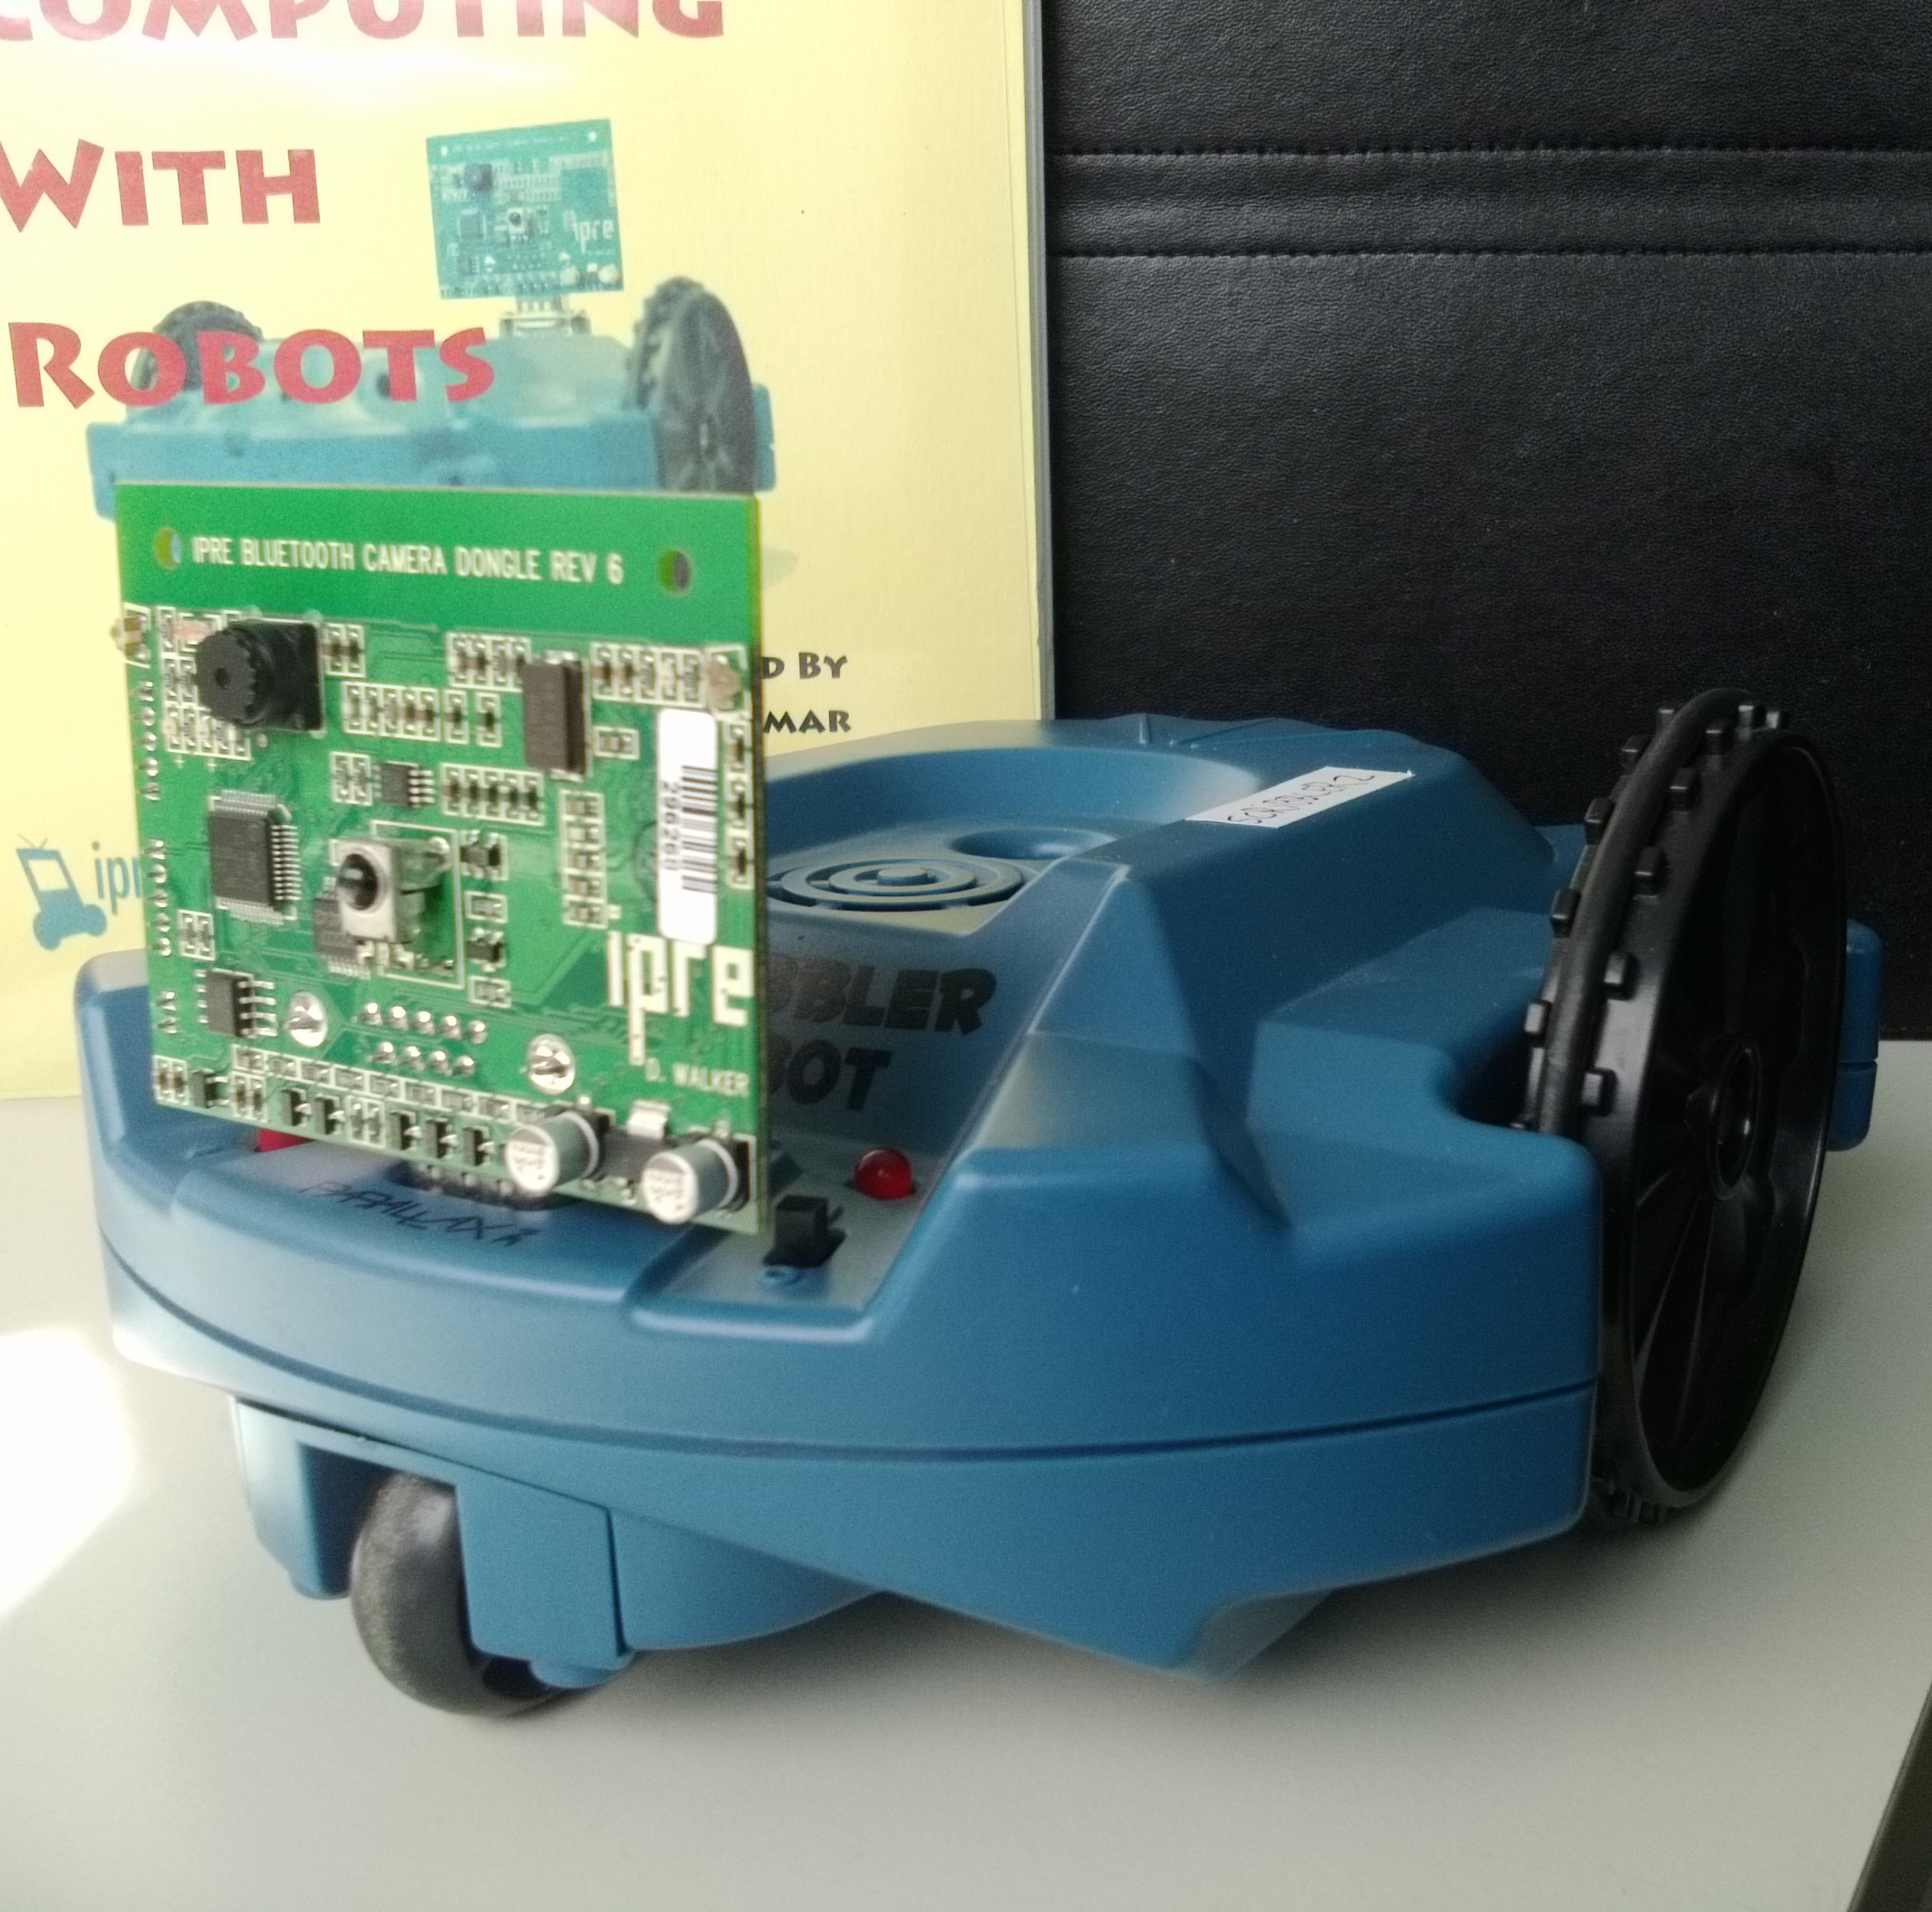
\includegraphics[width=\textwidth]{figures/scribbler}
        \subcaption{Robot Scribbler de Parallax}\label{fig:robots_usados_scribbler}
    \end{subfigure}
    \begin{subfigure}[b]{0.49\textwidth}
        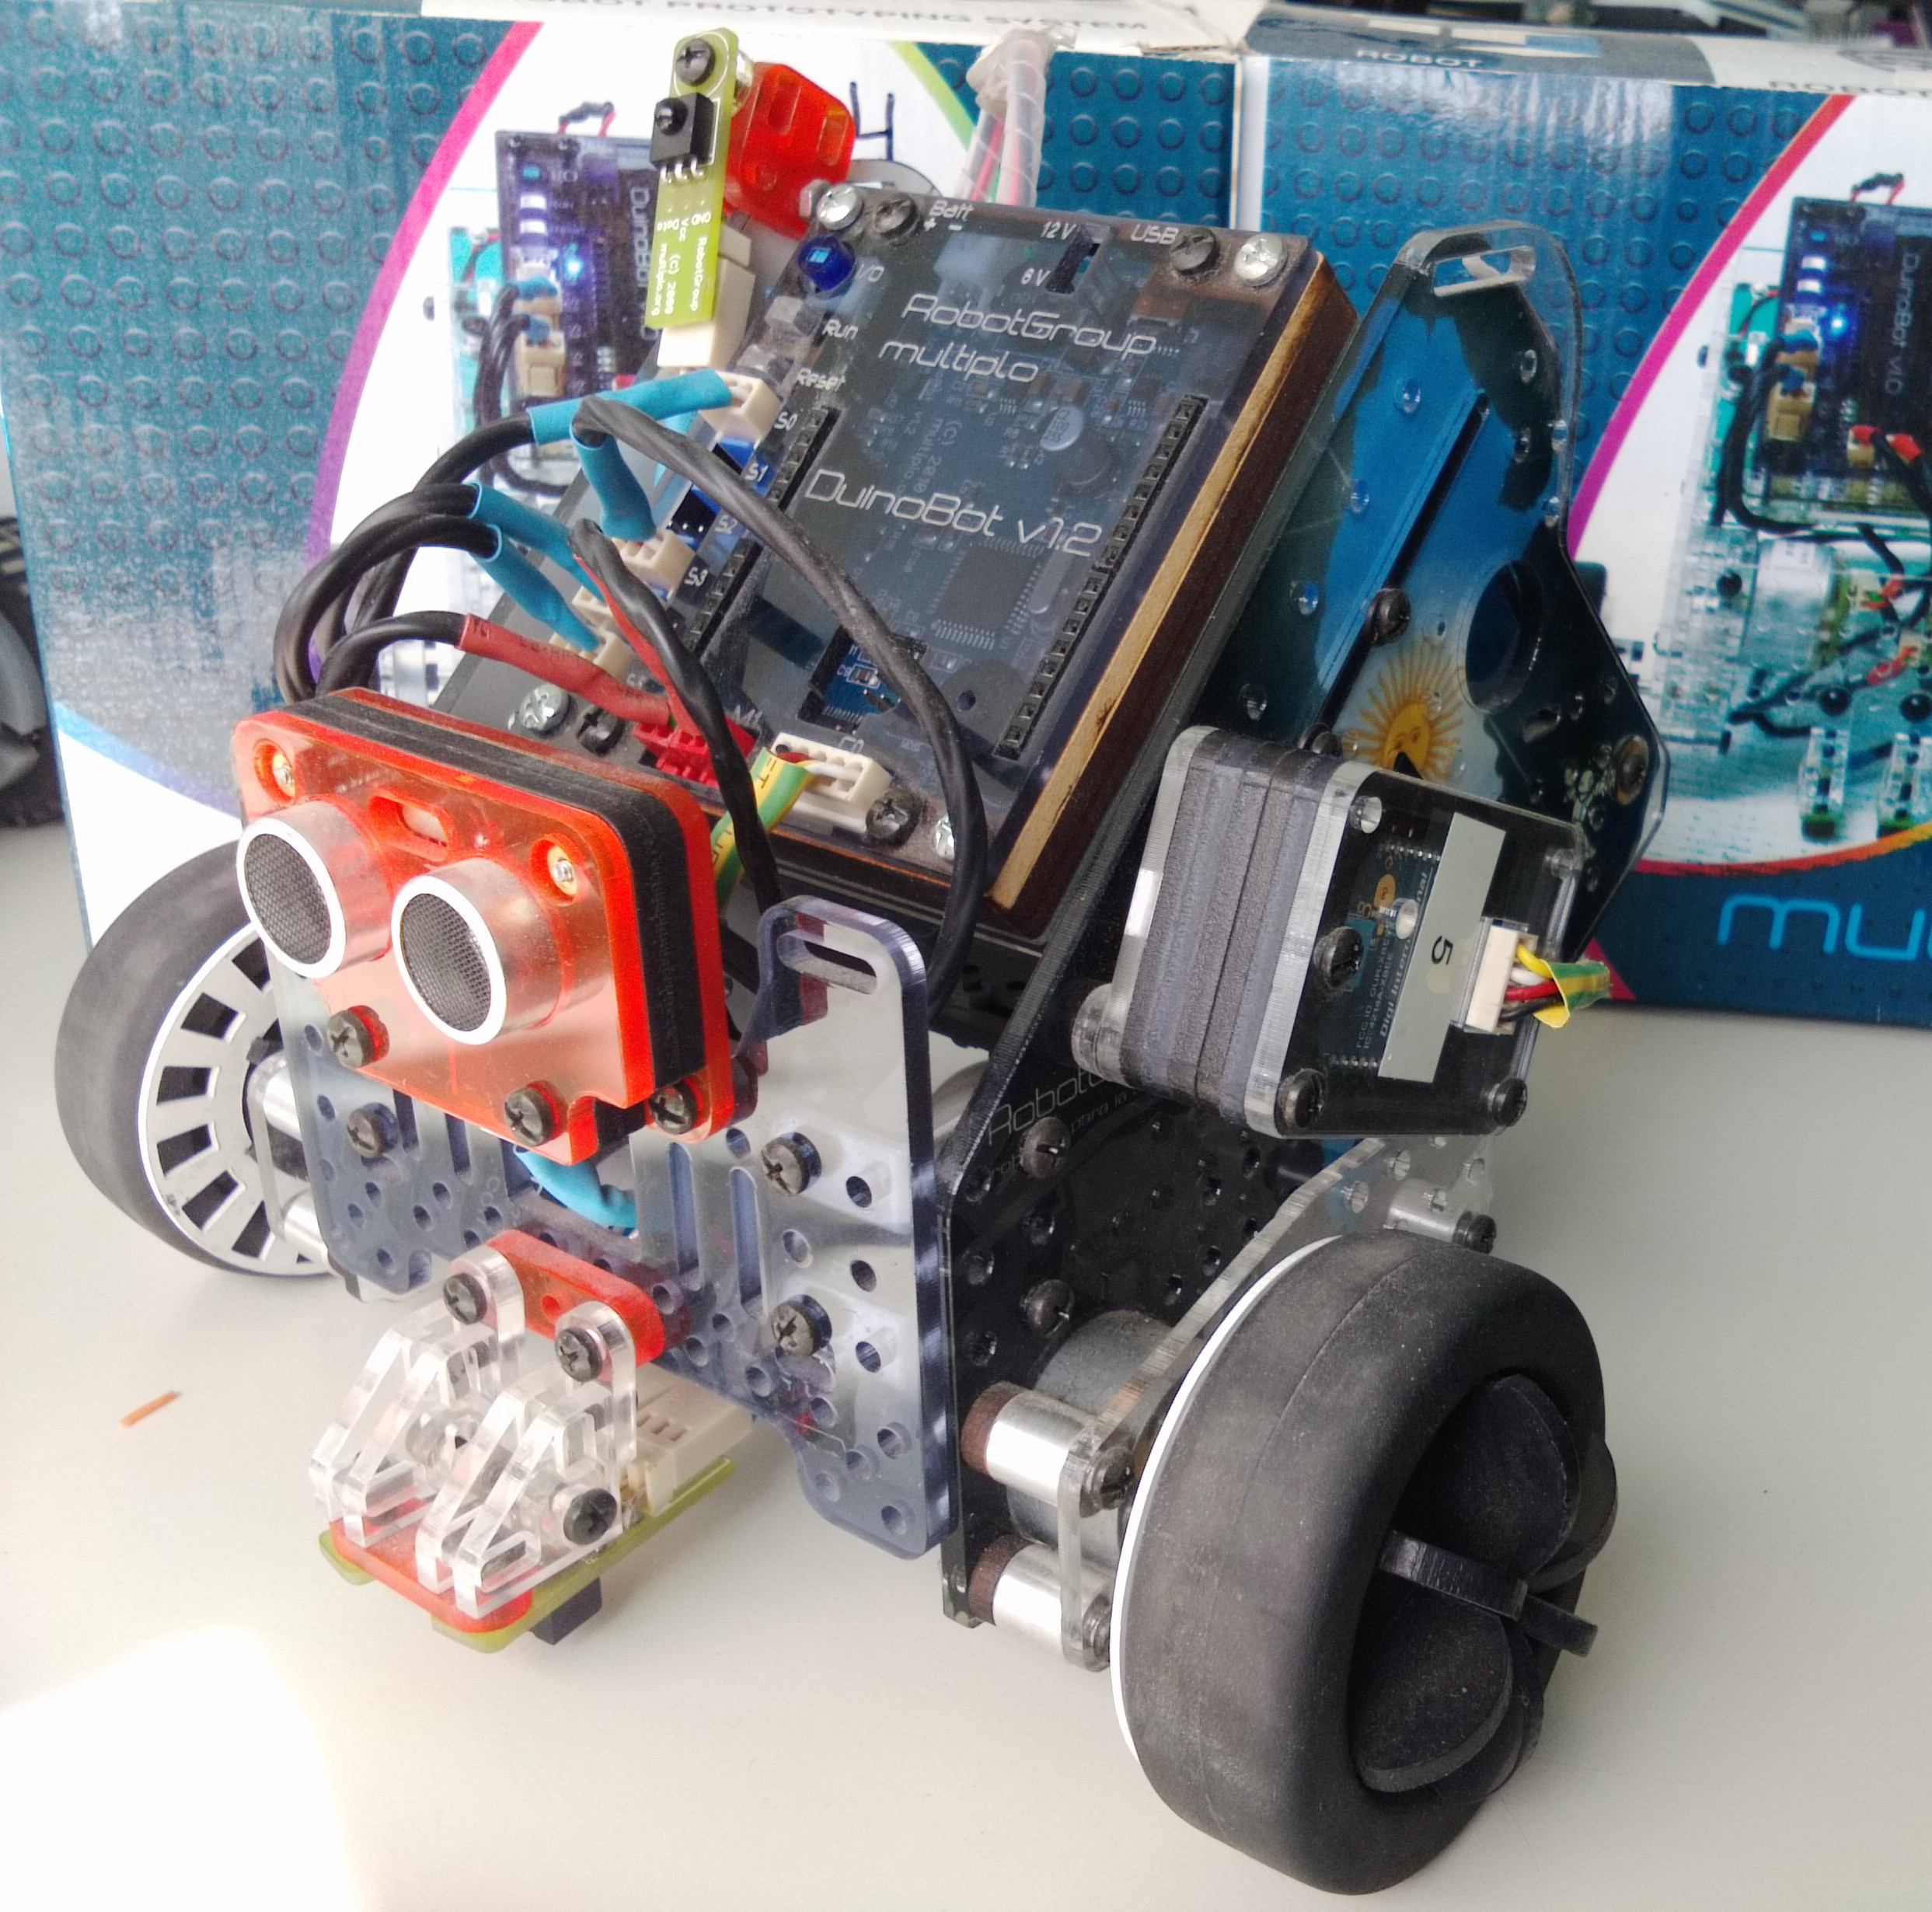
\includegraphics[width=\textwidth]{figures/n6}
        \subcaption{Robot Multiplo N6 de RobotGroup}\label{fig:robots_usados_n6}
    \end{subfigure}
    \caption{Robots usados en el proyecto}\label{fig:robots_usados}
\end{figure}

En un comienzo se utilizaron los robots Scribbler de Parallax, mostrados en
la figura~\ref{fig:robots_usados_scribbler}. Estos robots pueden programarse
directamente a través de un cable utilizando el lenguaje
PBASIC\footnote{\url{http://homepages.ius.edu/RWISMAN/C490/html/PythonandRobots.htm}
y\\ \url{http://learn.parallax.com/teach/pbasic-programming-basic-stamp}}
y funcionar de forma autónoma, o pueden ser controlados de forma
inalámbrica incorporando un dispositivo extra y conectándose por Bluetooth.

En las experiencias realizadas se los utilizó de
la última
forma, y de esta manera se controla el robot usando el lenguaje Python
(cuyo intérprete no
es posible ejecutar directamente sobre el microcontrolador del mismo).

Los robots Scribbler se importan desde Estados Unidos en volúmenes bajos
por las restricciones a la importación en nuestro país, lo que
dificulta su adquisición tanto por el equipo del proyecto como de posibles
escuelas que quisieran comprarlos, dejando, además al equipo sin ninguna
garantía
ante posibles averías. Por estos motivos, se buscaron alternativas de
fabricación nacional,
que pudieran ser programados en lenguaje Python y tuvieran especificaciones
abiertas.
De esta manera, a fines del año 2011, se adquirieron dos robots Multiplo N6
de fabricación nacional de
la empresa RobotGroup, mostrados en la figura~\ref{fig:robots_usados_n6}.
Tanto el software necesario para controlar estos robots como sus
especificaciones se distribuyen bajo una licencia
abierta\footnote{\url{https://www.kickstarter.com/projects/1689254125/multiplo-create-your-own-robot/description}}.

Los robots Multiplo N6 están basados en
Arduino\footnote{\url{http://www.arduino.cc/}}
por lo que pueden ser programados
usando el IDE Arduino en C++. Además RobotGroup ofrece el entorno de programación
MiniBloq que permite programar el robot de forma gráfica usando bloques.
Dado que estas modalidades no se adecuaban a las propuestas del proyecto
se pidió a la empresa una versión modificada del robot para controlarlo de forma
inalámbrica (ya que no es posible ejecutar un intérprete CPython en una
placa de esas características) y se
desarrolló
una biblioteca Python que permite la programación del robot en dicho lenguaje. Este
desarrollo fue realizado en forma conjunta entre el equipo del proyecto \proyecto{}
y miembros de la empresa RobotGroup, y actualmente está
siendo mantenido por el LINTI~\citep{diaz_aprendiendo_2012}.

La biblioteca Python que permite controlar los robots Multiplo N6 se
denomina DuinoBot. Se eligió este nombre por coincidir con el de la placa
controladora de los robots, sin embargo en este informe DuinoBot hace
referencia a la biblioteca Python desarrollada en conjunto
entre el equipo del proyecto \proyecto{} y la empresa RobotGroup.

En el año 2012, a través de un convenio de cooperación con la Fundación YPF,
que brindó
un subsidio, y bajo el auspicio de la Dirección de Escuelas Técnicas de la
Provincia de Buenos Aires se realizó una
capacitación en 10 escuelas técnicas de la
provincia de Buenos Aires. La Fundación YPF brindó a cada una de estas
escuelas, entre otras
cosas, 20 robots Multiplo N6 que quedaron en cada escuela. En estos cursos
se capacitaron más de 140 docentes y 40 alumnos avanzados, en programación
en el lenguaje Python utilizando
estos dispositivos~\citep{diaz_aprendiendo_2012} como herramienta didáctica.

Esta experiencia consolidó el uso de
los robots Multiplo N6 en el proyecto
``Programando con robots y software libre'', reemplazando
a los robots Scribblers, tanto por su confiabilidad como por su facilidad de
adquisición.

\section{Los robots}
Como se mencionó anteriormente, se utilizaron a lo largo del proyecto dos
modelos de robots distintos: el Scribbler y el Multiplo N6. Esta sección provee una
breve descripción de sus características técnicas.

\subsection{Robot Scribbler de Parallax}
Los robots Scribbler (versión 1) cuentan con un microcontrolador
\textit{PIC16F57}\footnote{Esta información se obtuvo con una inspección
visual de uno de estos robots.}
que viene programado con un intérprete de Basic. El producto
completo es denominado por Parallax
``Basic Stamp 2''\footnote{\url{http://www.andybrain.com/extras/scribbler-robot-review.htm}}.
Para su locomoción este robot cuenta con dos ruedas conectadas a través de
cajas
reductoras
a sus respectivos motores de DC (corriente continua)  y una tercer rueda no conectada a ningún
motor que sirve como tercer punto de apoyo para el cuerpo del robot.

La alimentación eléctrica del robot es provista por 6 pilas AA.

En cuanto a los sensores, este robot está equipado con:
\begin{itemize}
    \item Dos emisores infrarrojos a los lados de su parte frontal y un
        sensor infrarrojo entre ellos que permite sensar (de acuerdo a si se
        refleja el haz de luz infrarroja de alguno de los laterales) si
        hay algún obstáculo a la derecha o a la izquierda del robot.
    \item Tres fotorresistores ubicados dentro de 3 cavidades al frente del
        robot que permiten sensar la presencia de fuentes de luz e
        identificar (si la luz no es muy difusa) si las mismas se encuentran
        directamente enfrente, a la izquierda o a la derecha del robot.
    \item Dos sensores de línea que consisten cada uno de un emisor
        y un sensor infrarrojo (IR). Los mismos detectan cambios de contraste
        en el piso de acuerdo a la cantidad de luz IR reflejada y generalmente
        se utilizan para que el robot siga un camino demarcado por una línea
        de un color sobre una superficie de un color contrastante.
\end{itemize}

\begin{figure}
    \centering
    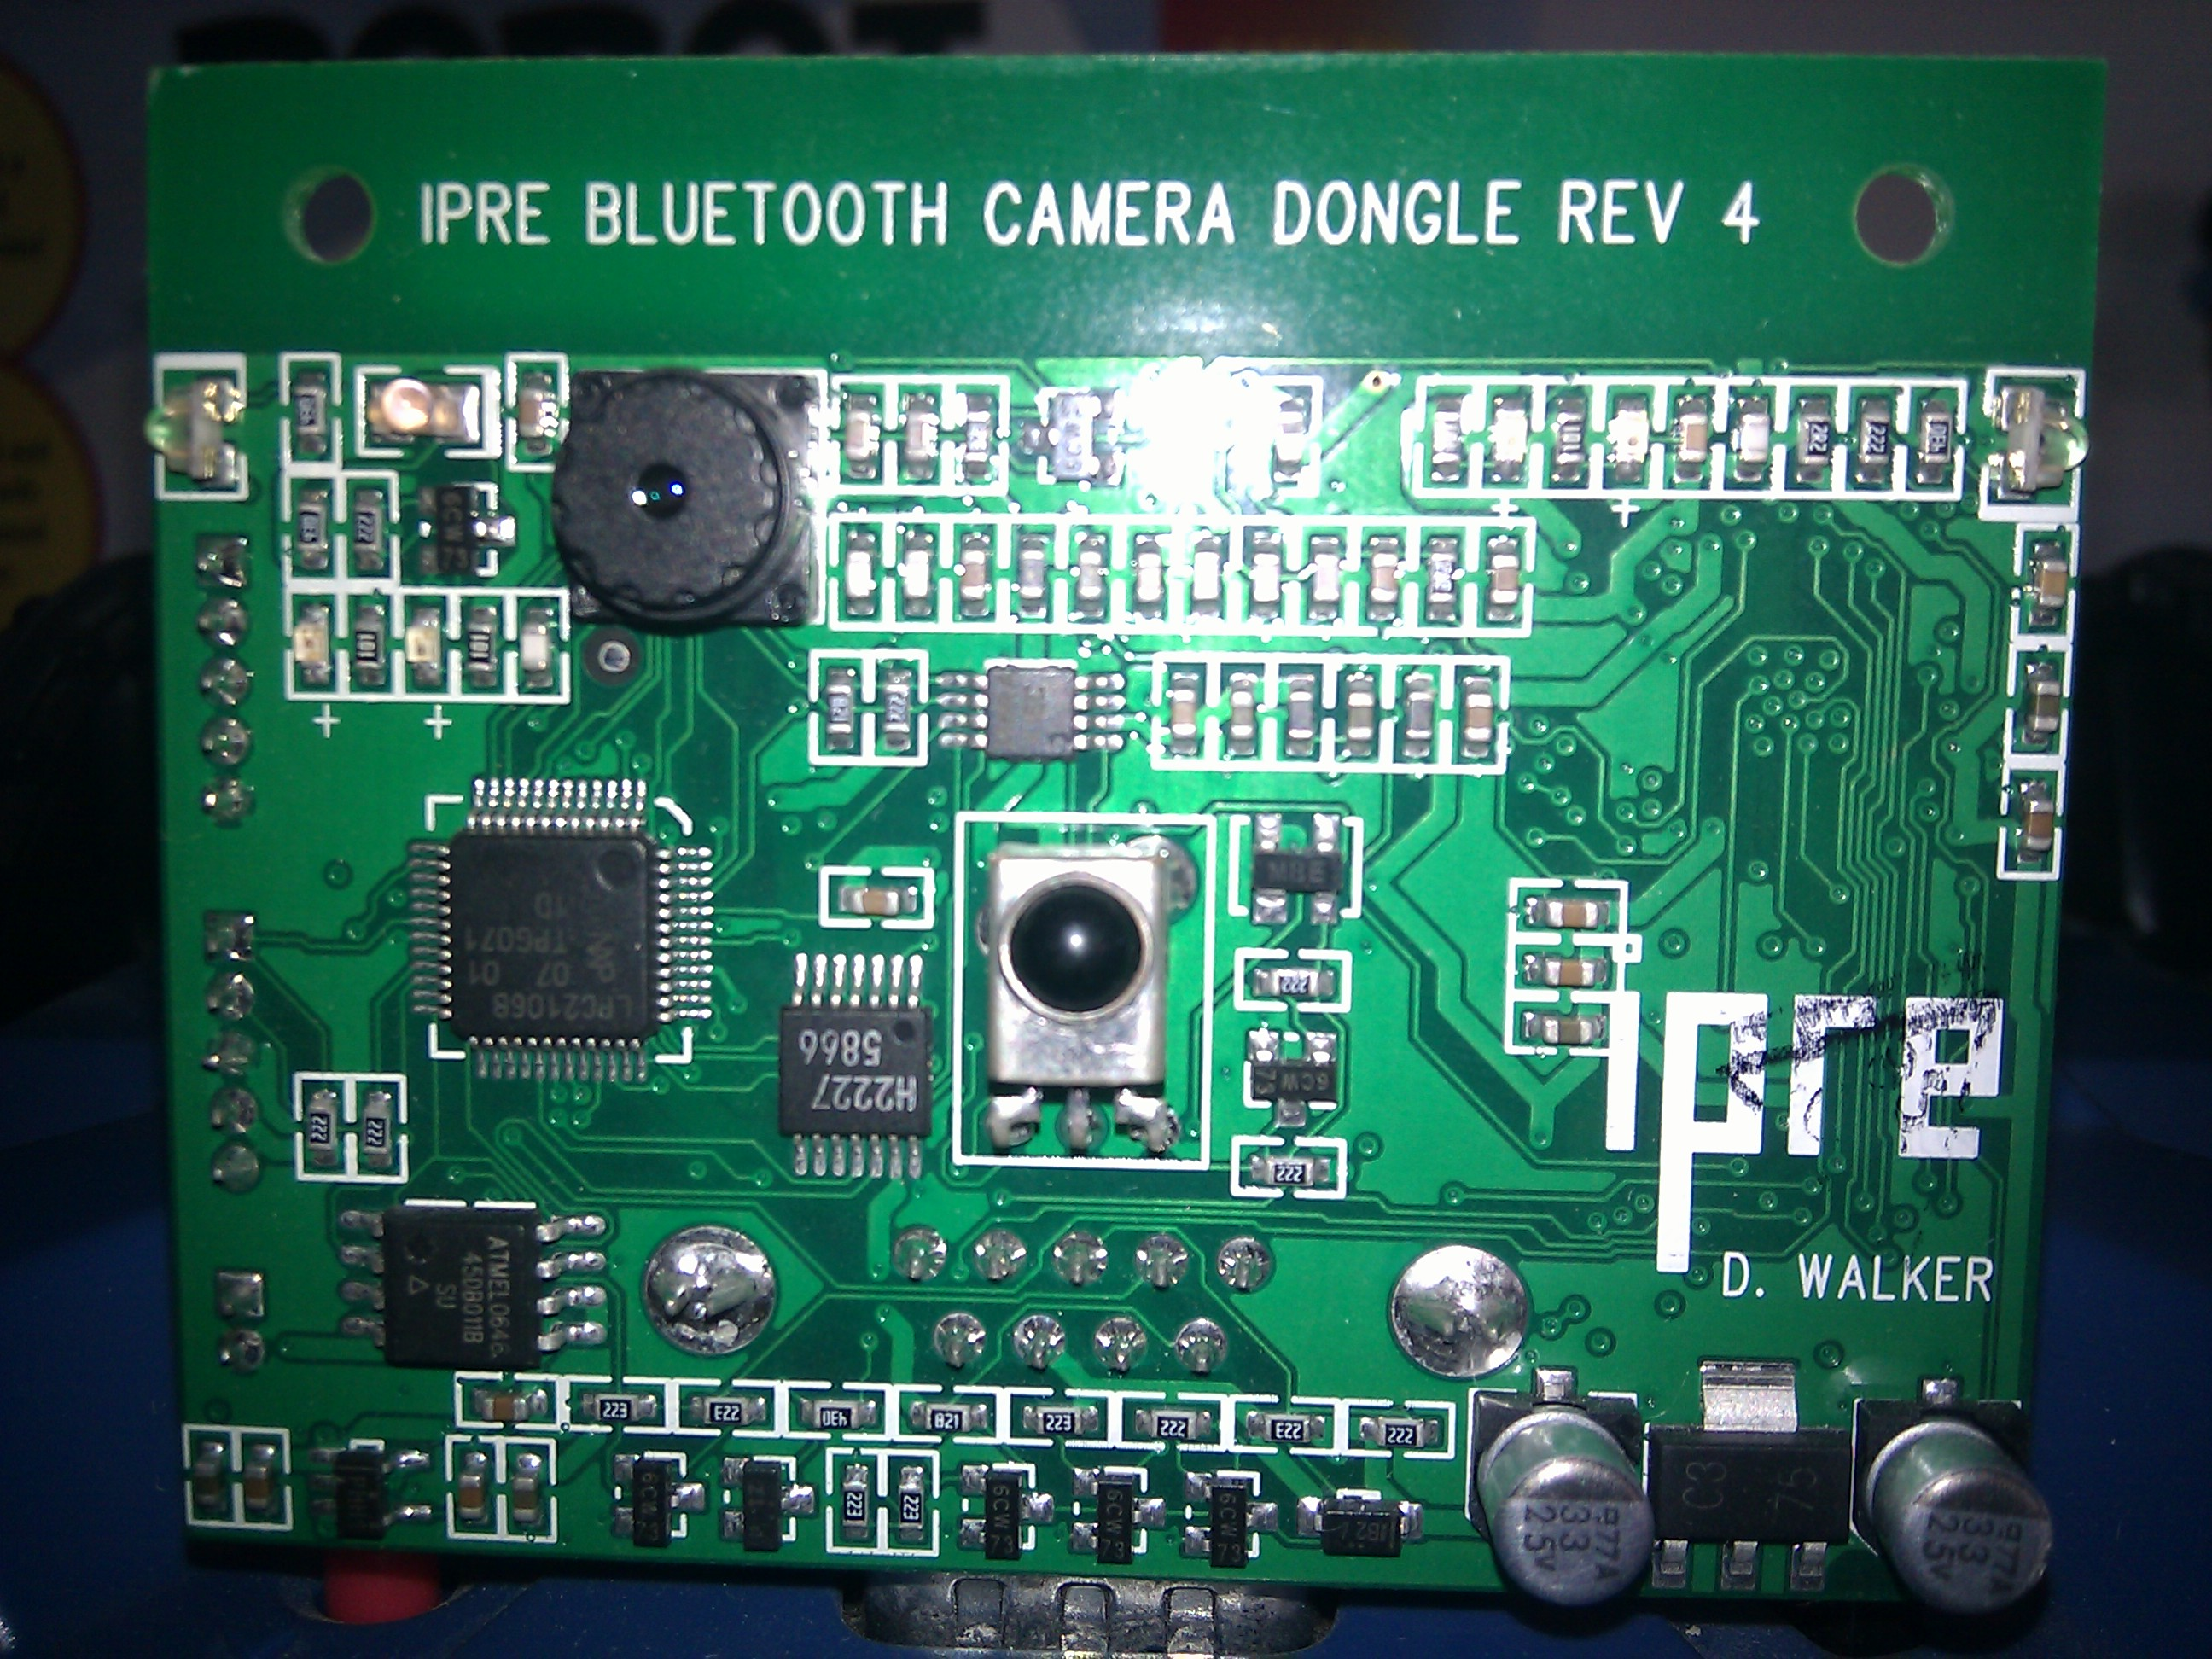
\includegraphics[width=0.5\linewidth]{figures/fluke}
    \caption{IPRE Fluke}
    \label{fig:foto_fluke}
\end{figure}

Si bien las anteriores son las características generales de estos robots, usándolos
de esta manera es necesario programarlos a través de un cable serial usando el
lenguaje PBASIC basado en BASIC. Para las actividades planteadas en el marco del
proyecto \proyecto{}, se utilizó  una versión
que agrega un dispositivo extra: el IPRE Fluke~\ref{fig:foto_fluke}.
Este dispositivo se conecta al puerto
serial del robot y provee la capacidad de controlarlo de forma inalámbrica
usando Bluetooth.  Conectar el
IPRE Fluke invierte el sentido de giro de las ruedas, por lo que el frente
del robot pasa a ser el lugar donde se conecta el IPRE Fluke. De aquí
en adelante cuando se mencione la parte delantera del Scribbler, será la
parte donde se encuentra conectado el IPRE Fluke y la parte trasera será la
opuesta.

El IPRE Fluke es comandado por con un microcontrolador
\textit{LPC2106F}\footnote{Información obtenida con una inspección visual
de la placa.}
basado en la arquitectura
\textit{ARM7}\footnote{\url{http://pdf1.alldatasheet.com/datasheet-pdf/view/83950/PHILIPS/LPC2106FHN48.html}}. Posee un módulo de comunicaciones
Bluetooth que utiliza como medio de comunicación con la computadora
controlante y
provee una cámara de baja resolución con la que se pueden tomar fotografías,
que luego serán transmitidas por Bluetooth. Además agrega
un sensor infrarrojo que permite detectar la presencia de obstáculos
a la izquierda, al centro o a la derecha (está compuesto de 3 emisores
y un
receptor)\footnote{\url{http://wiki.roboteducation.org/Myro_Hardware}}.
Con esta incorporación el robot queda equipado ahora con sensores
en la parte frontal y en la parte trasera, pero más importante aún
el módulo Bluetooth permite controlarlo de forma inalámbrica siempre
que se grabe un firmware especial en la placa IPRE Fluke. Esto es lo que permite
que estos robots puedan ser programados con Python usando una biblioteca denominada
\textit{Myro}\footnote{\url{http://wiki.roboteducation.org/Myro_Reference_Manual}},
que será descripta en la sección~\ref{sec:myro}.

\subsection{Multiplo N6}
El robot Multiplo N6, fabricado por la empresa RobotGroup, cuenta con un
microcontrolador Atmel
\textit{AVR ATMega32U4}\footnote{\url{http://www.robotgroup.com.ar/index.php/productos/131-robot-n6\#especificaciones}}
con el bootloader de Arduino
precargado. Para su locomoción cuenta con dos ruedas conectadas a través
de reductores de velocidad a sus correspondientes motores de
corriente continua y una tercer
rueda no conectada a ningún motor que sirve como tercer punto de apoyo.
La alimentación eléctrica de estos robots está dada por tres pilas AA
en serie (o bien dos packs de tres pilas cada uno en paralelo).

En cuanto a los sensores el Multiplo N6 está equipado con:
\begin{itemize}
    \item Un sensor ultrasónico para detectar obstáculos al frente del
        robot.
    \item Un sensor infrarrojo que puede ser utilizado en conjunto con
        un control remoto universal para enviar comandos al robot
        (siempre que se programe este comportamiento previamente).
    \item Dos sensores detectores de línea, compuestos de un emisor y
        un receptor infrarrojo cada uno. Opcionalmente estos sensores
        pueden desatornillarse y ensamblarse
        para funcionar como
        ``encoders''\footnote{\url{http://machinedesign.com/sensors/basics-rotary-encoders-overview-and-new-technologies-0}}
        de las ruedas y de esta manera es posible
        calcular la velocidad de giro de las ruedas. Este uso
        no es recomendable si se controla el robot de forma remota
        ya que la latencia de las comunicaciones puede hacer que se pierdan
        datos haciendo que el cálculo de la velocidad sea impreciso.
\end{itemize}

En esta configuración estos robots son programables usando el entorno de
Arduino y desde MiniBloq\footnote{\url{http://minibloq.org}}, pero dado que el objetivo del proyecto es la enseñanza de
programación en el lenguaje Python se encargó a la empresa una versión
modificada del Multiplo N6 que permitiera controlarlo de forma inalámbrica,
de manera tal que una computadora con un intérprete de Python instalado
pudiera enviar instrucciones y recibir los valores de los sensores
del robot tal como hace la biblioteca Myro con los robots Scribbler.
Esta
modificación consistió en la adición de un módulo de comunicación inalámbrica
XBee
que permite enviar y recibir datos del robot a través del protocolo
ZigBee\footnote{\url{http://www.digi.com/xbee/}}, la modificación de
un firmware basado en una implementación existente para Arduino del protocolo
de control \texttt{Firmata}\footnote{\url{http://firmata.org/}} y el
desarrollo
del módulo Python \texttt{DuinoBot} para controlar a los robots usando
este protocolo, el
cuál fue adaptado por los miembros del proyecto \proyecto{}
para soportar nuevas funcionalidades y proveer una
API similar a la de la biblioteca
\texttt{Myro}\citep{lanfranco_2012}.

Básicamente los robots Multiplo N6 utilizados en el proyecto \proyecto{}
contienen un
firmware basado en Firmata, modificado para soportar
las características propias del robot. Este firmware recibe instrucciones desde
un un puerto serie conectado a una placa XBee y envía las respuestas
a la misma utilizando una variación del protocolo Firmata. Desde el lado
de la computadora controlante, el módulo DuinoBot provee una interfaz
de alto nivel para los alumnos, donde cada instrucción para el robot
programada
en Python se convierte a una secuencia de bytes del protocolo Firmata
y se envía al robot a través de una placa XBee conectada por USB a la
computadora, y cada respuesta del robot se almacena para ser utilizada
como valor de respuesta en los métodos asociados con los sensores.


\section{Características comunes}
Aunque se han utilizado a la fecha estos dos modelos distintos de robots,
en esencia, las características principales de ambos modelos son las mismas
y coinciden con las de otros robots usados en la Argentina para enseñar a
programar. En general, todos ellos incluyen:
\begin{itemize}
    \item Un medio de locomoción  con 2 motores continuos que mueven cada
        uno una de las ruedas laterales.
    \item Sensores que permiten detectar obstáculos.
    \item Sensores que permiten detectar líneas.
    \item Operación inalámbrica.
\end{itemize}

Cabe destacar sobre este último ítem que otros robots no requieren
cables para operar ya que son programados
a través de algún lenguaje compilado como C, Assembler
o Basic, donde se les transfiere el programa a través de un
cable (usualmente USB o Serial)
y este programa se graba en la memoria del microcontrolador permitiendo
que el robot posteriormente ejecute el programa de forma autónoma.
Pero los robots usados en el proyecto antes mencionado no requieren
cables ya que son controlados a través de señales
inalámbricas, lo que permite controlarlos en tiempo real y utilizando
un intérprete Python estándar (CPython) instalado en el dispositivo
controlante.

Dado el costo y fragilidad de los robots habitualmente los alumnos interactúan
con los mismos solamente en el aula, ya sea en su escuela si la misma
adquirió los robots, o en las instalaciones de la  Facultad de Informática si el alumno
realiza alguna pasantía o práctica en la misma. Esto tiene varias connotaciones:
\begin{itemize}
    \item El alumno, al estar en una situación formal en la escuela
        compartiendo el robot (recurso limitado) con otros
        alumnos, posiblemente no tenga el tiempo o el ambiente más apropiado
        para experimentar de forma lúdica con el mismo.
    \item La tarea para casa solamente es realizable a través de un simulador
        que puede ser lo suficientemente completo y fiel como para aprender
        a programar, pero resulta menos estimulante y realista que manipular
        un robot real.
    \item Alumnos de escuelas que no tienen los recursos necesarios para
        adquirir el equipamiento o de escuelas alejadas de
        la ciudad de La Plata, que
        no tienen la posibilidad de acercarse a nuestra
        Facultad, no pueden interactuar con robots reales
        (a lo sumo podrán usar un simulador).
\end{itemize}

Por otro lado, las placas
XBee que permiten conectarse con los robots Multiplo N6
son relativamente costosas. El esquema normal de conexionado entre dispositivos
controladores y robots descripto en el capítulo~\ref{cha:myro_y_duinobot}
requiere
2 placas XBee por robot, una conectada directamente al robot y la otra
conectada por USB al dispositivo controlante. En consecuencia:
\begin{itemize}
    \item El dispositivo controlante debe tener un puerto USB y los drivers
        necesarios para detectar la interfaz serial con el XBee, esto deja
        fuera de juego celulares y tablets.
    \item El costo de operar cada robot en este esquema es sensiblemente
        superior al costo que tendría si varios alumnos pudieran
        controlar varios robots usando un solo dispositivo XBee compartido
        entre varios dispositivos controlantes.
\end{itemize}

Tomando estos dos problemas se propuso implementar una solución
que permita
superarlos de forma simultánea. Esta solución permite controlar los
robots a través de una red, como puede ser Internet, permitiendo a los alumnos
conectarse a los robots desde sus hogares y a las instituciones a compartir
el uso de sus robots. Por otro lado también es posible configurar el servidor
para su uso en el aula deshabilitando funcionalidades innecesarias en un ámbito
local, como ser la necesidad de autenticar a los usuarios para utilizar los
robots. Este modo de operación fue pensado para que múltiples alumnos puedan
acceder a múltiples robots contando con un solo adaptador USB a XBee. Esto
reduciría sensiblemente el costo de cada robot por alumno ya que de otra
manera por cada robot deberían usarse 2 dispositivos XBee (uno en el robot
y otro en la computadora del alumno) reduciéndose con este modo de operación
a un XBee por robot más un único adaptador USB a XBee conectado al servidor.

Como consecuencia de estos requerimientos el servidor
debe tener una interfaz web y proveer acceso concurrente, con relativa
baja latencia, para permitir a múltiples alumnos acceder a múltiples robots
al mismo tiempo desde distintos dispositivos.
Si bien el objetivo del proyecto \proyecto{} es enseñar
programación usando el lenguaje Python, por lo que sería suficiente
que XRemoteBot tenga un cliente Python, tener un servidor web basado en
protocolos estándares hace que sea relativamente sencillo desarrollar
clientes en cualquier lenguaje
que soporte estos protocolos. Esto dio lugar a la posibilidad de
implementar otros clientes que permitieran usar los robots para enseñar
programación en distintos lenguajes sin reimplementar el protocolo
de bajo nivel. XRemoteBot se diseñó de forma tal que la creación
de nuevos clientes en distintos lenguajes resulte sencilla.
En especial, la elección de protocolos y tecnologías usadas
y la falta de necesidad de acceder directamente al hardware a través de USB,
habilita la implementación de un cliente Javascript que se ejecute en el
navegador web de los usuarios. Esta implementación, junto con las desarrolladas
en Ruby y Python, se describen en el capítulo~\ref{cha:clientes}, y permite
trabajar con el robot desde un navegador web.

El nivel de abstracción que puede proveer esta API hace que sea
una consecuencia natural de este diseño pensar
en la posibilidad de manejar distintos tipos de robots
que tengan algunas características mínimas en común con los robots ya
descriptos utilizando la misma interfaz de programación. Por lo que
teniendo ciertos cuidados en la implementación del protocolo y el
servidor se puede lograr que ambos sean fácilmente extensibles para
agregar soporte para nuevos robots.

En cuanto al lenguaje de programación utilizado en el desarrollo del servidor,
dado que las bibliotecas utilizadas para controlar los robots Multiplo N6 y
Scribbler se encuentran desarrolladas en Python y dada la experiencia del autor
tanto en el uso de estas bibliotecas como en el uso del lenguaje Python en general,
éste es el lenguaje elegido para el desarrollo del servidor. En particular la
versión 2.7 de Python ya que utilizar la versión 3 requeriría extensivas
modificaciones a estas bibliotecas y otras relacionadas~\citep{lutz_2014}.

\appendix
% Apéndice A Serialización

\chapter{Serialización}
\label{ch:serializacion}

Siendo una aplicación cliente-servidor remotebot requiere algún método de
serialización para intercambiar datos entre los clientes y el servidor,
considerando que el servidor no es más que un servidor web que usa websockets
como protocolo, el método de serialización más adecuado parece ser JSON
(Javascript Serialization Object Notation).

JSON cuenta con las siguientes características:

\begin{enumerate}
    \item Es un formato estandarizado por ECMA~\citep{ecma-404}
        y está especificado por la rfc-7159~\citep{rfc-7159}.
    \item Soporta los tipos de datos necesarios para intercambiar mensajes con
        los datos necesarios para controlar los robots usando un nivel de
        abstracción adecuado.
    \item Al ser un formato de texto es simple analizar el tráfico entre los
        clientes y el servidor para detectar posibles errores.
    \item Está soportado de forma nativa por los navegadores más
        utilizados%~\footnote{\url{http://caniuse.com/#search=json}}.
\end{enumerate}

Pero también existen otras alternativas cuyos objetivos son serialización
y de-serialización rápida, y datos serializados más compactos
como BSON (Binary JSON) y (CBOR Concise Binary Object Representation).

Algunas características de BSON y CBOR son:

\begin{enumerate}
    \item Codifican la información en formato binario.
    \item Son tan fáciles de usar como JSON.
    \item Ambos formatos proveen un superset de los tipos de datos provistos
        por JSON.
    \item CBOR está especificado por la rfc-7049~\citep{rfc-7049}.
    \item BSON tiene una especificación informal pero cuenta una
        implementación bien conocida siendo la representación de datos primaria en
        MongoDB~\footnote{\url{http://bsonspec.org/}}.
    \item Por estar en formato binario decodificar una captura de tráfico
        para depurar un programa es más laborioso.
    \item En algunos casos estos formatos binarios generarán mensajes más
        chicos que JSON, pero no siempre.
    \item Requieren usar librerías Javascript en los clientes web ya que los
        navegadores no lo implementan de forma nativa.
\end{enumerate}

Para tomar un decisión respecto al formato a utilizar se decidió generar
16 archivos \texttt{JSON} con datos aleatorios, estos archivos se cargaron
con una cantidad de entradas múltiplo de 1024 desde 1024 hasta 16384, donde
cada una de estas entradas es un objeto \texttt{JSON} con 5 entradas de tipo
numérico, 5 strings, 5 objetos (cada uno con una entrada numérica) y 5
arrays (cada uno con 2 entradas de tipo string).

Estos archivos se cargaron desde scripts similares en Python y Javascript que
de-serializaron y serializaron estos datos repetidas veces calculando el tiempo
promedio que llevó hacer cada una de estas acciones para cada formato.

Se eligió hacer las pruebas con Python y Javascript porque el primero es el
lenguaje de implementación del servidor y del cliente que probablemente tenga
más uso en un futuro, mientras que Javascript es el lenguaje de implementación
del cliente que se ejecutará en los navegadores web y que puede servir como
base para implementaciones con Brython, Skulp, Opal, etc...

Para hacer el experimento repetible la implementación en
Javascript se ejecutó con el intérprete \textbf{nodejs} basado en
el motor \textbf{v8} usado por \textbf{Chrome} y además se crearon
scripts de apoyo para generar los datos de prueba, ejecutar los scripts
con los distintos formatos de forma automatizada y formatear los datos
resultantes en archivos csv.

Todas las pruebas se realizaron sobre Lihuen 6 beta (basado en Debian Jessie)
en una notebook con procesador ``Intel(R) Core(TM) i3 CPU M 370 @ 2.40GHz''
y 4GB de RAM % NOTA: son 4GB no 4GiB
usando Python 3.4.2 y NodeJS 0.10.35~\footnote{Se usó NodeJS 0.10.35 ya que
la versión 0.10.29 distribuida al momento con Debian Jessie tenía un bug que
generaba un error de memoria al
deserializar strings largos con \texttt{JSON.load} (CVE-2014-5256)}

De estas pruebas se desprenden las mediciones de las
figuras~\ref{fig:ser-time-py}, \ref{fig:ser-time-js} y \ref{fig:ser-size}.

\begin{figure}
    \centering
    \begin{framed}
        \begin{tikzpicture}[trim axis left, trim axis right]
            \begin{axis}[
                    height=10cm,
                    width=10cm,
                    scaled x ticks = false, % No usar notación exponencial
                    xlabel=Cantidad de entradas,
                    ylabel=Segundos,
                    x tick label style={/pgf/number format/fixed, rotate=45, anchor=north east}, % Las etiquetas son números y rotar 45°
                    xtick=data, % Generar una etiqueta por punto en los datos
                    ylabel near ticks, % Poner las etiquetas más o menos cerca de algunos datos
                    ymin=0, % No hay tiempos negativos
                    xmin=1024, % La escala empieza en 1024
                    legend style={legend pos=north west}, % Cuadro de leyendas a la derecha arriba
                    every axis x label/.style={
                        at={(axis description cs:0.5,-0.15)}, % Desplazar la descripción del eje x
                        anchor=north, % El desplazamiento relativo a la parte superior del texto
                    },
                    legend cell align=left, % Alineación del texto en la caja de leyendas
                ]
                \foreach \s in {json, bson, cbor} {
                    \addlegendentryexpanded{\s\ dump}
                    \addplot table [x=entries, y=dump_time, col sep=comma] {data/py-\s.csv};

                    \addlegendentryexpanded{\s\ load}
                    \addplot table [x=entries, y=load_time, col sep=comma] {data/py-\s.csv};
                }
            \end{axis}
        \end{tikzpicture}
    \end{framed}

    \caption{Cantidad de entradas versus tiempo de serialización y deserialización en Python}
    \label{fig:ser-time-py}
\end{figure}

\begin{figure}
    \centering
    \begin{framed}
        \begin{tikzpicture}[trim axis left, trim axis right]
            \begin{axis}[
                    height=10cm,
                    width=10cm,
                    scaled x ticks = false, % No usar notación exponencial
                    xlabel=Cantidad de entradas,
                    ylabel=Segundos,
                    x tick label style={/pgf/number format/fixed, rotate=45, anchor=north east}, % Las etiquetas son números y rotar 45°
                    xtick=data, % Generar una etiqueta por punto en los datos
                    ylabel near ticks, % Poner las etiquetas más o menos cerca de algunos datos
                    ymin=0, % No hay tiempos negativos
                    xmin=1024, % La escala empieza en 1024
                    legend style={legend pos=north west}, % Cuadro de leyendas a la derecha arriba
                    every axis x label/.style={
                        at={(axis description cs:0.5,-0.15)}, % Desplazar la descripción del eje x
                        anchor=north, % El desplazamiento relativo a la parte superior del texto
                    },
                    legend cell align=left, % Alineación del texto en la caja de leyendas
                ]
                \foreach \s in {json, bson, cbor} {
                    \addlegendentryexpanded{\s\ dump}
                    \addplot table [x=entries, y=dump_time, col sep=comma] {data/js-\s.csv};

                    \addlegendentryexpanded{\s\ load}
                    \addplot table [x=entries, y=load_time, col sep=comma] {data/js-\s.csv};
                }
            \end{axis}
        \end{tikzpicture}
    \end{framed}
    \caption{Cantidad de entradas versus tiempo de serialización y deserialización en Javascript (nodejs)}
    \label{fig:ser-time-js}
\end{figure}


\begin{figure}
    \centering
    \begin{framed}
        \begin{tikzpicture}[trim axis left, trim axis right]
            \begin{axis}[
                    height=10cm,
                    width=10cm,
                    scaled x ticks = false,
                    xlabel=Cantidad de entradas,
                    ylabel=Tamaño en MiB,
                    x tick label style={/pgf/number format/fixed, rotate=45, anchor=north east},
                    xtick=data,
                    ylabel near ticks,
                    ymin=0,
                    xmin=1024,
                    legend style={legend pos=north west},
                    every axis x label/.style={
                        at={(axis description cs:0.5,-0.15)},
                        anchor=north,
                    },
                    legend cell align=left
                ]
                \foreach \s in {json, bson, cbor} {
                    \addlegendentryexpanded{\s}
                    \addplot table [x=entries, y=serialized_size, col sep=comma] {data/js-\s.csv};

                }
            \end{axis}
        \end{tikzpicture}
    \end{framed}
    \caption{Cantidad de entradas versus tamaño del archivo serializado}
    \label{fig:ser-size}
\end{figure}

De la figura~\ref{fig:ser-size} se desprende que los distintos métodos de
serialización no ofrecen diferencias significativas en el tamaño de los
strings generados para los volumenes de datos probados. Por otro lado
se puede observar en la figura~\ref{fig-ser-time-py} que al menos en
Python y con la librería usada CBOR tiene los mejores tiempos, sin
embargo en las pruebas con Javascript en la figura~\ref{fig:ser-time-js}
se puede observar que los mejores tiempos son para el formato JSON,
esto es entendible ya que este es el único formato procesado de forma
nativa~\footnote{Si bien es posible encontrar parsers nativos para los
otros formatos y usarlos desde NodeJS no se utilizó esta modalidad porque
no sería una prueba realista dado que los motores Javascript de los
navegadores no permiten esto.}.

Teniendo en cuenta que las diferencias de tiempo al procesar los datos
en Python son, en comparación con la versión en Javascript, marginales
(apenas alrededor de $0.25$ segundos para $2^{14}$
entradas entre el mejor y peor tiempo de deserialización) y las diferencias
en cuanto a tamaño del string generado al
serializar también son pequeñas (aproximadamente 2MiB de diferencia para
$2^{14}$ entradas entre el mejor y el peor método

%% This defines the bibliography file (main.bib) and the bibliography style.
%% If you want to create a bibliography file by hand, change the contents of
%% this file to a `thebibliography' environment.  For more information 
%% see section 4.3 of the LaTeX manual.
\begin{singlespace}
\bibliography{main}
\bibliographystyle{apalike}
\end{singlespace}

\end{document}

